\documentclass[conference]{IEEEtran}
\usepackage{graphicx}

\begin{document}

\title{Realization of Fine-grained Sequential Approximate Circuits using Fault Emulation}


\author{\IEEEauthorblockN{BLIND REVIEW}
\IEEEauthorblockA{}
\and
\IEEEauthorblockN{BLIND REVIEW}
\IEEEauthorblockA{}
}


% make the title area
\maketitle


\begin{abstract}
%\boldmath
Approximate Computing has recently drawn interest due to its promise to substantially decrease the power consumption of integrated circuits. By tolerating a certain incorrectness at a circuit output, it can be operated at a more resource-saving state. For instance, parts of the circuit could be switched off or driven at sub-threshold voltage. Clearly, not all applications are suitable for this approach. Especially applications from the signal and image processing domain are suitable, due to their intrinsic tolerance to imprecision. But even in these circuits, one has to be very careful when and where to approximate a circuit, in order not to violate a minimum QoS.\\
In this paper we are presenting a complete approach to generate approximate circuits from existing deterministic implementations. The flow reaches from application-driven QoS definition down to approximated RTL. We are using FPGA-based fault emulation of the circuit in order to find out how faults, i.e. imprecisions in the circuit, affect the circuit behavior.\\
Most existing approaches only consider combinational circuits. Compared to existing approaches considering sequential circuits, our approach is very fast and accurate due to the FPGA-based emulation. And furthermore, we are able to tune the resulting precision to the defined QoS, in order to bring out the best gain of the approximation.
\end{abstract}

\IEEEpeerreviewmaketitle



\section{Introduction}
\subsection*{Approximate Computing}
\subsection*{Related Work}






\section{Methodology}
\subsection{faultify - Probability-aware Fault Emulation}
\subsection{Application-reasoned Approximation }
\begin{figure}[htb]
  \centering
  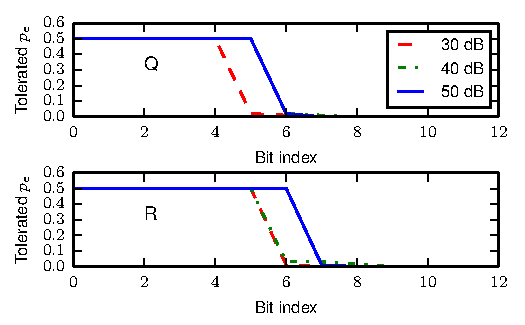
\includegraphics[width=.5\textwidth]{figs/metrics_qr}
  \caption{Tolerable imprecision of a QR decomposition, part of a 8x8 MIMO zero-forcing equalizer, for different signal qualities and a target BER=$0.01$}
  \label{fig:metrics_qr}
\end{figure}
\begin{figure}[htb]
  \centering
  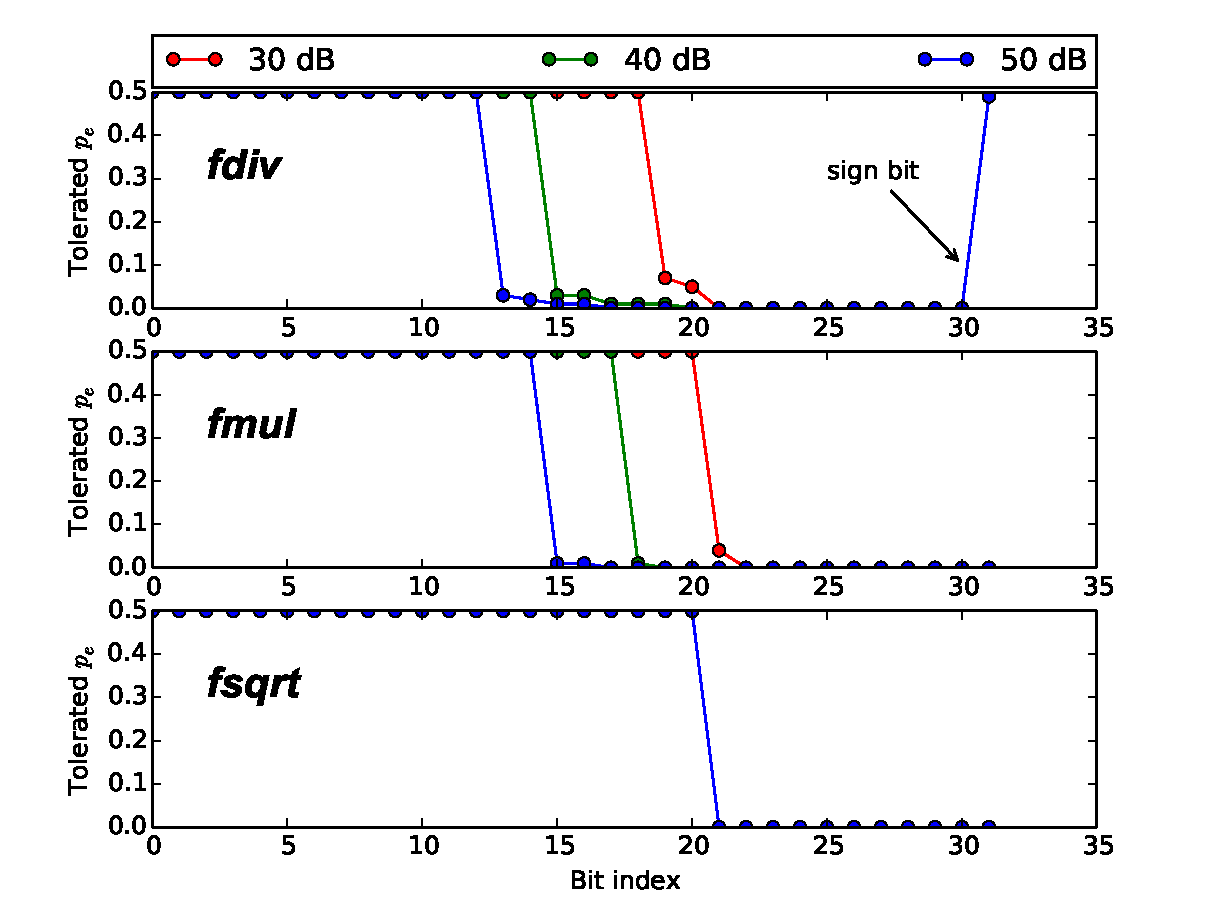
\includegraphics[width=.5\textwidth]{figs/metrics_sobel}
  \caption{Tolerable imprecision of a \emph{sobel} filter for different target qualities (PSNR)}
  \label{fig:metrics_sobel}
\end{figure}
\subsection{Approximation of Sequential Circuits}
% Hier keine Figures, verweis auf exp. results

















\section{Experimental Results}
\begin{tabular} {| l | l | c | c |}
\hline
Name & Description & Gates & Flip-flops \\
\hline\hline
FIR & 16-tap FIR filter & xx & xx \\
IIR & 8-tap IIR filter & xx &xx \\
DCT4 & 4-input DCT & xx & xx \\
DCT8 & 8-Input DCT & xx & xx \\
fpu100 & 32-bit floating point unit & xx & xx \\
QR & QR decomposition & xx & xx \\
vitdec & Viterbi decoder (131,81) & xx & xx \\
\hline
\end{tabular}
\subsection{Energy/Area}
\subsubsection{FPGA target}
\subsubsection{ASIC target}















\section{Conclusion}






\section*{Acknowledgment}





% trigger a \newpage just before the given reference
% number - used to balance the columns on the last page
% adjust value as needed - may need to be readjusted if
% the document is modified later
%\IEEEtriggeratref{8}
% The "triggered" command can be changed if desired:
%\IEEEtriggercmd{\enlargethispage{-5in}}

% references section
\bibliographystyle{IEEEtran}
\bibliography{IEEEabrv,islped}





% that's all folks
\end{document}


